\chapter{Prototype Implementation}
\label{ch:prototype}

Following the successful design and characterization of the custom actuator module, the research progresses
to the system-level integration. This chapter details the physical assembly of the modular robotic limb and
the establishment of the control infrastructure required to bridge the simulation environment with the real
world.

The primary objective of this phase is to validate the mechanical design and the kinematic control strategies
derived in Chapter \ref{ch:model} under real-world conditions. The validation relies on a
Hardware-in-the-Loop (HIL) architecture, which allows for direct comparison between the theoretical model
and the physical prototype.

The scope of these experiments is strictly limited to the verification of the kinematic model and trajectory tracking
capabilities in an open-loop configuration. The proprioceptive and adaptive control strategies discussed in Section
\ref{sec:proprioception}, while validated in simulation, are excluded from this experimental verification due to
project time constraints.

\section{Hardware-in-the-Loop Architecture}

The successful implementation of the prototype relies on the seamless integration of the mechanical hardware
with the control software. To bridge the theoretical environment (MATLAB/Simulink) with the physical reality, a
Hardware-in-the-Loop (HIL) architecture was established. This approach allows the complex kinematic algorithms
to run on the host PC, while a dedicated embedded bridge manages the low-level communication with the distributed
actuator network.


\subsubsection{Physical Assembly}

The mechanical structure of the limb was realized through additive manufacturing (3D printing) using the CAD
models developed during the design phase. The structural links (Coxa, Femur, Tibia) were printed in PLA to
ensure an optimal stiffness-to-weight ratio.

These components were assembled with the three newly designed custom actuator modules described in Chapter
\ref{ch:servomotor} (see Figure \ref{fig:limb_assembly}). A critical design feature introduced in this assembly is
the axis extension mechanism. To mitigate the radial stress on the servo output shaft an idler bearing was integrated
into the frame opposite to the motor shaft. This configuration effectively creates a simply supported beam structure,
significantly increasing mechanical stability.

\begin{figure}[htbp]
    \centering
    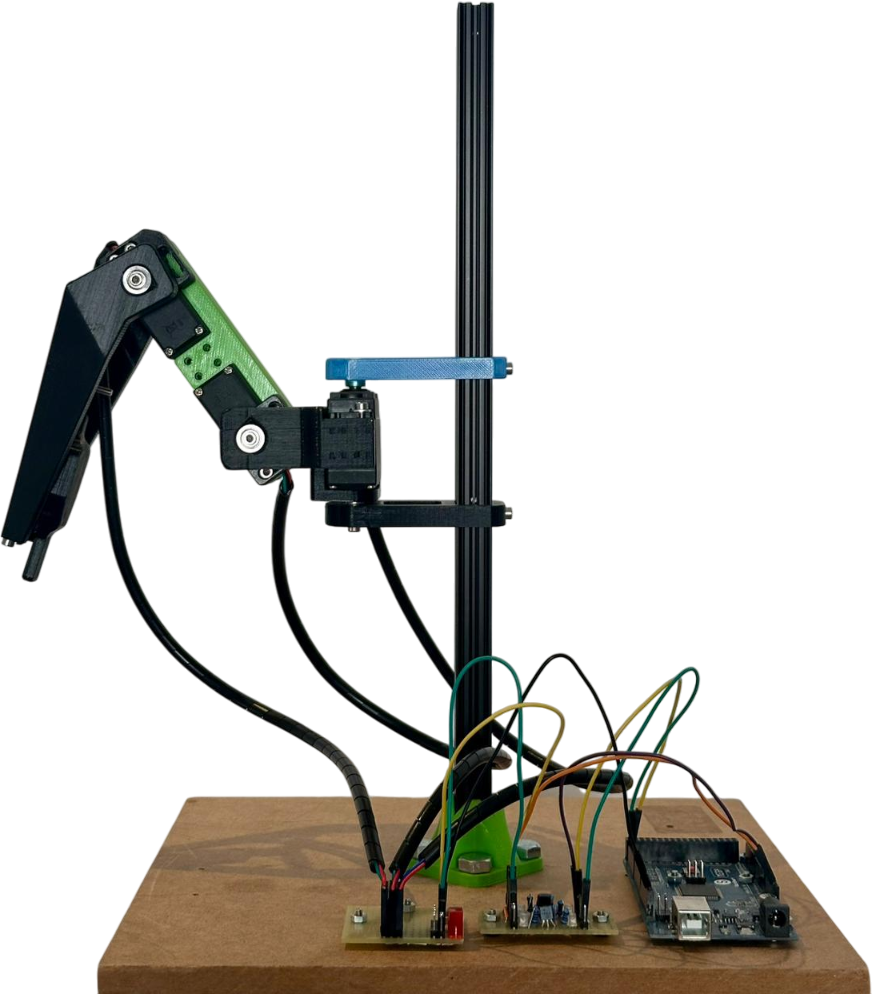
\includegraphics[width=0.88\textwidth]{images/limb_assembly.png}
    \caption{Mechanical Assembly of the Prototype Limb.}
    \label{fig:limb_assembly}
\end{figure}

With the exception of the custom actuator housings and fasteners, the physical limb geometrically coincides perfectly
with the numerical model used in the simulations (Section \ref{sc:simulation}), providing a first visual
confirmation of the prototype's fidelity.


\subsubsection{Simulink/Arduino Control Environment}

The Simulink model, originally developed for pure digital simulation, acts as the High-Level Controller. The
"Leg Model (Plant)" block used in Chapter \ref{ch:model} is replaced by a Serial Interface Block. This modified
control scheme (Figure \ref{fig:hil_scheme}) operates as follows:

\begin{enumerate}
    \item Generation and Transmission: The Path Planner and Inverse Kinematics blocks generate the reference
        joint angles $q_d$ in real-time. These references are quantized and transmitted via USB-Serial to the
        microcontroller bridge.
    \item Hardware Bridge: The interface between the host PC and the actuator network is managed by an Arduino
        board (Arduino Mega 2560). The firmware sketch, parses the UART data and forwards the position setpoints
        to the actuator network via $\text{I}^2\text{C}$ bus. Immediately after it queries their current position
        (also via $\text{I}^2\text{C}$). Then the received data ($q_{hw}$) is transmitted back to Simulink.
    \item Feedback Loop: After the return packet containing the measured joint angles $q_{hw}$ arrives, the
        feedback data is fed into the Forward Kinematics block to reconstruct the actual end-effector position
        $p_{hw}$ for performance analysis.
\end{enumerate}

\begin{figure}[htbp]
    \centering
    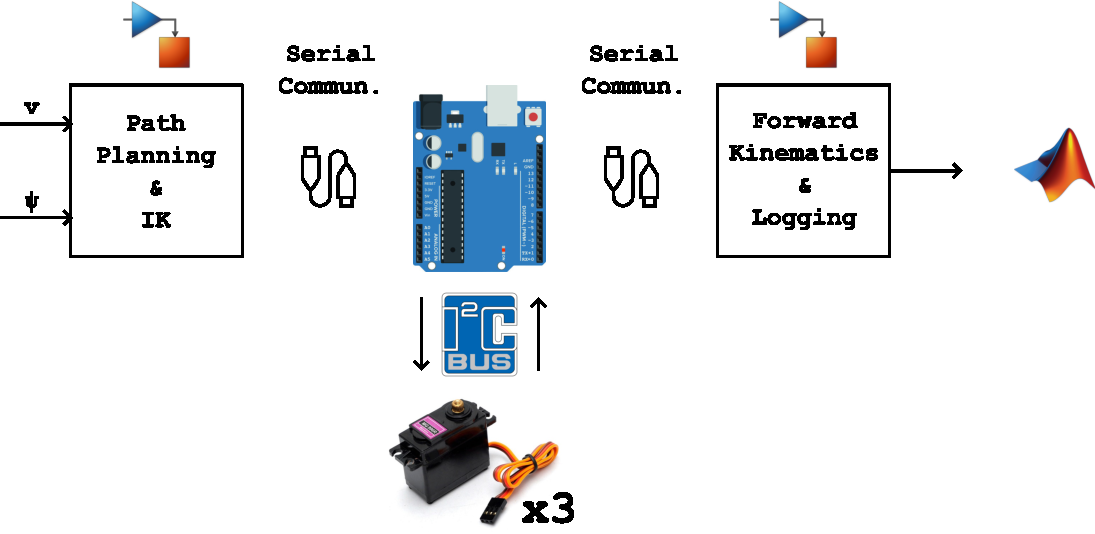
\includegraphics[width=0.9\textwidth]{images/hil.pdf}
    \caption{Block Diagram of the Hardware-in-the-Loop Control Architecture.}
    \label{fig:hil_scheme}
\end{figure}


\subsubsection{Experimental Protocol}

To ensure a rigorous validation, the experimental setup is designed to strictly mirror the conditions of the
digital simulation presented in Chapter \ref{ch:model}. The reference input for the physical limb is the exact
same $C^2$ continuous gait trajectory derived in Section \ref{sec:trajectory}.

The real-time control chain operates at a fixed update frequency of $100\,\text{Hz}$ ($\Delta t = 10\,\text{ms}$).
In each cycle, the Simulink High-Level Controller samples the continuous trajectory, computes the inverse
kinematics solution $q_d$, and transmits the packet to the embedded bridge. Synchronously, the actual joint
positions $q_{hw}$ are acquired from the actuators and logged.

The primary objective of this experiment is to quantify the \textit{Sim-to-Real} gap by overlaying the
experimental data on the simulation results.
\section{Performance Assessment and Results}

The following results provide a quantitative comparison between the reference command ($p_d$, $q_d$), the
simulated response ($p_{sim}$, $q_{sim}$), and the actual experimental telemetry ($p_{hw}$, $q_{hw}$).


\subsubsection{Cartesian Trajectory Tracking}

Figure \ref{fig:gait_z_psi_exp} illustrates the side-view trajectory ($Z\psi$-plane) of the end-effector. Visual
inspection confirms that the physical limb successfully replicates the desired gait profile. The stance phase remains
reasonably flat, while the swing phase achieves the target clearance height without significant deviation. Crucially,
the experimental path (orange) remains close to the Optimal Workspace Region (dotted line), validating the
safety margins established during the design phase.

\begin{figure}[htbp]
    \centering
    
\includegraphics[width=0.65\textwidth]{images2/gait_z_psi.pdf}
    \caption{Experimental Gait Trajectory in the $Z\psi$-plane (Side View).}
    \label{fig:gait_z_psi_exp}
\end{figure}

Figure \ref{fig:gait_spacetime} shows the time evolution of the trajectory in a 3D graph. Several persistent
perturbations can be seen along the path. This is attributed to model calculation lags on the simulink side,
as they appear during the FSM path generator state transition, and also to external force (gravity).

\begin{figure}[htbp]
    \centering
    
\includegraphics[width=0.65\textwidth]{images2/gait_3d_spacetime.pdf}
    \caption{Experimental Gait Trajectory in Space-Time.}
    \label{fig:gait_spacetime}
\end{figure}

A time-domain analysis of the Cartesian coordinates is provided in Figure \ref{fig:cart_traj_exp}. The experimental
tracking shows a high degree of fidelity, with all the coordinates closely following the command. The $X$ coordinate,
which should ideally remain constant, shows minor fluctuations ($< 2$ mm) negligible for locomotion stability, while
the $Y$ (propulsion) and $Z$ (lift) components exhibit a small tracking delay. This is expected due to the discrete
nature of the control loop.

\begin{figure}[htbp]
    \centering
    \begin{subfigure}[b]{0.8\textwidth}
        \centering
        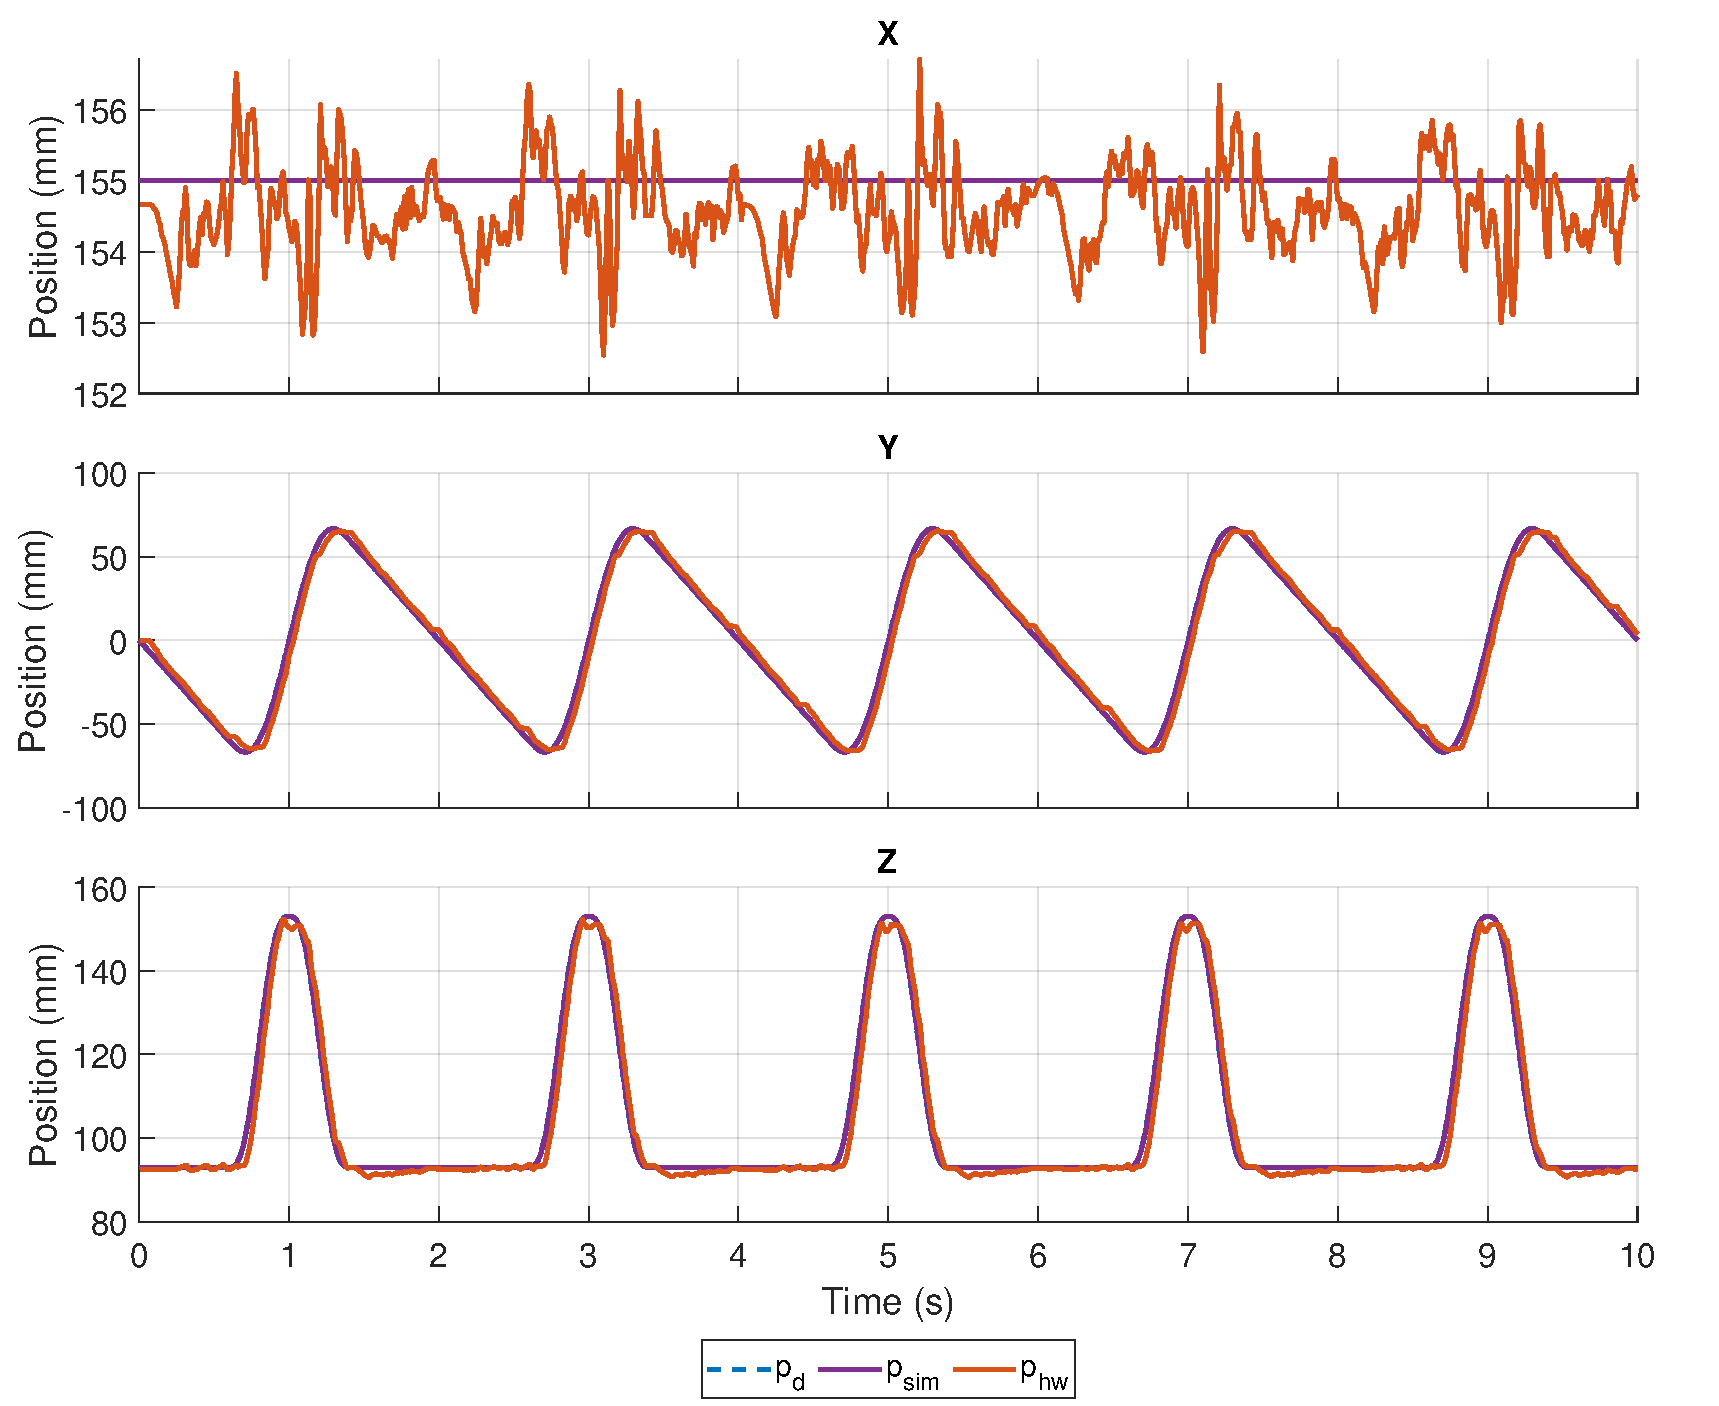
\includegraphics[width=\textwidth]{images2/cartesian_trajectories.pdf}
        \caption{Trajectory Tracking}
        \label{fig:cart_traj_exp}
    \end{subfigure}

    \begin{subfigure}[b]{0.8\textwidth}
        \centering
        
\includegraphics[width=\textwidth]{images2/cartesian_errors.pdf}
        \caption{Tracking Errors}
        \label{fig:cart_err_exp}
    \end{subfigure}
    \caption{Cartesian-Space Experiment Results.}
    \label{fig:cart_exp}
\end{figure}

The error plot (Figure \ref{fig:cart_err_exp}) reveals similarities in the simulation and experimental error shapes,
fundamentally changing only in amplitude (refer also to Figure \ref{fig:joint_results} for better understanding).
The amplitude difference can be attributed to a higher tracking delay, while the shape of the error is reasonably
due to inertial effects, purposely neglected at this stage of control.


\subsubsection{Joint Space Performance}

The performance at the actuator level is detailed in Figures \ref{fig:joint_traj_exp} and \ref{fig:joint_err_exp},
where once again it is visible how all three joints ($q_1, q_2, q_3$) track their respective references with
remarkable precision (also in this instance, the Simulation and Experimental plots differ by amplitude rather than
shape).

\begin{figure}[htbp]
    \centering
    \begin{subfigure}[b]{0.8\textwidth}
        \centering
        
\includegraphics[width=\textwidth]{images2/joint_trajectories.pdf}
        \caption{Trajectory Tracking}
        \label{fig:joint_traj_exp}
    \end{subfigure}

    \begin{subfigure}[b]{0.8\textwidth}
        \centering
        
\includegraphics[width=\textwidth]{images2/joint_errors.pdf}
        \caption{Tracking Errors}
        \label{fig:joint_err_exp}
    \end{subfigure}
    \caption{Joint-Space Experiment Results.}
    \label{fig:joint_exp}
\end{figure}


\subsubsection{Delay and Response Analysis}

To isolate the dynamic performance from the temporal evolution to promote a better visualization of the mentioned
tracking delay, Figure \ref{fig:tracking_delay_exp} presents the input-output correlation (Command vs. Measured
angle) for each joint. An ideal behaviour should be represented by a straight line ($y = x$), while a wider ellipse
would correspond to a higher tracking delay.

Both datasets populates the graph as expected (narrow ellipses for simulation and wider ellipses for the experiment).
Additionally, the slightly wider loops for $q_2$ and $q_3$ correlate with a higher inertial load due to gravity.

\begin{figure}[htbp]
    \centering
    \begin{subfigure}[b]{0.40\textwidth}
        \centering
        
\includegraphics[width=\textwidth]{images2/q_track_1.pdf}
        \caption{Hip ($q_1$)}
    \end{subfigure}
    \begin{subfigure}[b]{0.40\textwidth}
        \centering
        
\includegraphics[width=\textwidth]{images2/q_track_2.pdf}
        \caption{Knee ($q_2$)}
    \end{subfigure}

    \begin{subfigure}[b]{0.40\textwidth}
        \centering
        
\includegraphics[width=\textwidth]{images2/q_track_3.pdf}
        \caption{Ankle ($q_3$)}
    \end{subfigure}
    \caption{Tracking Delay Analysis.}
    \label{fig:tracking_delay_exp}
\end{figure}


\subsubsection{Quantitative Benchmark}

Unexpectedly, the tracking quality performs surprisingly well, despite the fact that the custom servomotor control
algorithm is originally designed for P2P control.

Ultimately, the tracking quality is quantified using the Root Mean Square Error (RMSE) metric (as per Section
\ref{sec:limitations}). Figure \ref{fig:rmse_benchmark} compares the simulation baseline against the physical
prototype.

While the experimental errors are naturally higher than the idealized simulation, the general trend matches for the
two cases, following similar magnitude patterns. The Cartesian RMSE is dominated by the Y-axis ($\approx 5.4$ mm),
consistent with the direction of maximum movement and backlash accumulation.
The main contributor to these errors in the experimental case, as shown in the previous section, was the tracking
delay. Nevertheless, the error remains however remarkably small for a low-cost prototype.

This quantitative benchmark conclusively validates the design approach: the custom actuators and the kinematic
model perform within the requirements defined at the outset of this thesis and well within acceptable limits for
stable locomotion.

\begin{figure}[htbp]
    \centering
    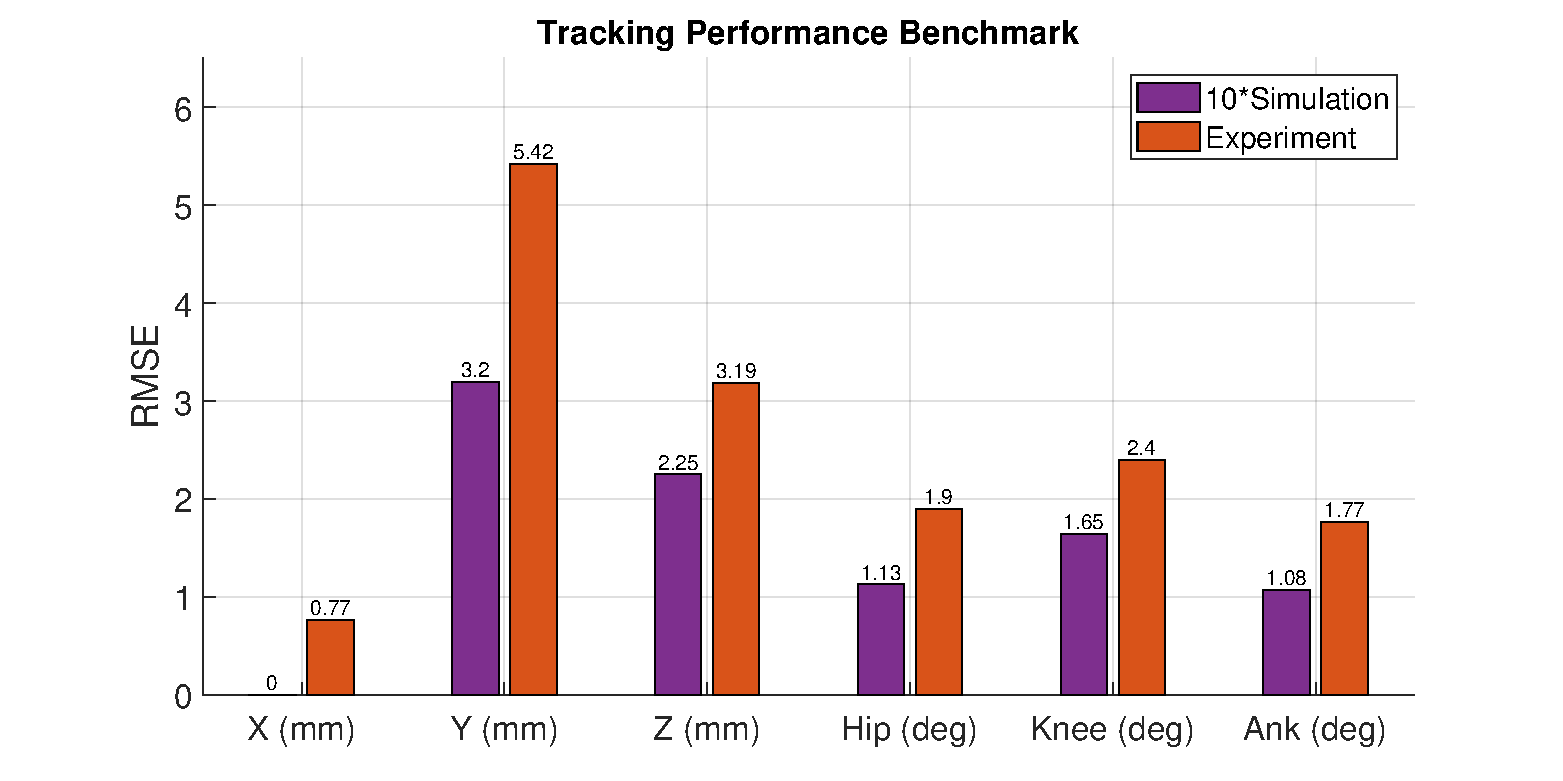
\includegraphics[width=0.98\textwidth]{images/rmse_benchmark.pdf}
    \caption{Simulation vs. Experiment Tracking Error.}
    \label{fig:rmse_benchmark}
\end{figure}
